% -*- coding: utf-8 -*-

% 配置宏包和订制环境
\documentclass[%
    %showsectionnum, %每节开头显示第几节编号
    %plainthanks, %空白致谢页
]{banyuan-ppt}

%添加自己要用到的宏包
%\usepackage{forest}
\usepackage{caption}
\captionsetup{font=scriptsize,labelfont=scriptsize}

\let\oldfootnotesize\footnotesize
\renewcommand*{\footnotesize}{\oldfootnotesize\tiny}

\usepackage[slide,linesnumbered,algoruled]{algorithm2e}
\DontPrintSemicolon
%\SetNlSty{\small\rm}

\usepackage{listings}

\usepackage{xcolor}

\definecolor{dkgreen}{rgb}{0,0.6,0}
\definecolor{gray}{rgb}{0.5,0.5,0.5}
\definecolor{mauve}{rgb}{0.58,0,0.82}

\lstdefinestyle{myScalastyle}{
  frame=tb,
  aboveskip=3mm,
  belowskip=3mm,
  showstringspaces=false,
  columns=flexible,
  basicstyle={\scriptsize\ttfamily},
  numbers=left,                    % where to put the line-numbers; possible values are (none, left, right)
  numbersep=-5pt,                   % how far the line-numbers are from the code
  numberstyle=\tiny\color{gray},
  keywordstyle=\color{blue},
  commentstyle=\color{dkgreen},
  stringstyle=\color{mauve},
  frame=single,
  breaklines=true,
  breakatwhitespace=true,
  tabsize=3,
}


% 文首
\begin{document}

% 封面
% -*- coding: utf-8 -*-

\title{GBDT、TreeBoost和XGBoost}
\subtitle{树模型的进化之路}
\author{颜发才 \\
        \href{mailto:facai.yan@gmail.com}{\tiny facai.yan@gmail.com} \\[-1ex]
        \href{https://facaiy.github.io}{\tiny facaiy.github.io}}
\institute{新浪微博算法平台}
\date{\today}

\createtitle

\begin{frame}
    \begin{figure}[!tb]
        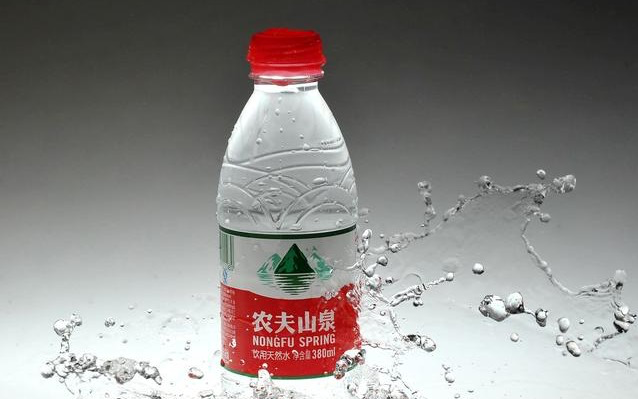
\includegraphics[width=1.2\onepicwidth]{figure/water}
        \caption{我们不生产水,我们只做大自然的搬运工\footnote{
                 \href{http://sh.qihoo.com/pc/967ac7a2370f8fc79?sign=360_e39369d1}{图片来源:快资讯}}}
    \end{figure}
\end{frame}

\begin{frame}{整体方向}
    \begin{itemize}
        \item 提高易用性
            \begin{itemize}
                \item eager execution
                \item tf.data
                \item tf.keras
                \item tf.functions
            \end{itemize}
        \item 用户代码模块化
            \begin{itemize}
                \item 移除全局变量
                \item 迁移和统一到tf.keras
            \end{itemize}
        \item 清理重复和老旧设计
    \end{itemize}
\end{frame}

% 目录
\createoutline

% 正文
% 大纲
% -*- coding: utf-8 -*-

\section{整体方向}

\begin{frame}{整体方向}
    \begin{itemize}
        \item 提高易用性
            \begin{itemize}
                \item eager execution
                \item tf.data
                \item tf.keras
                \item tf.functions
            \end{itemize}
        \item 用户代码模块化
            \begin{itemize}
                \item 移除全局变量
                \item 迁移和统一到tf.keras
            \end{itemize}
        \item 清理重复和老旧设计
    \end{itemize}
\end{frame}

%% -*- coding: utf-8 -*-

\subsection{tf.Variable}

\begin{frame}[fragile]{tf.Variable}
    \begin{tcblisting}{title=RefVariable的读写顺序问题}
        a = tf.Variable(1.0, use_resource=True)
        a.initializer.run()

        assign = a.assign(2.0)
        with tf.control_dependencies([assign]):
          b = a.read_value()
        with tf.control_dependencies([b]):
          other_assign = a.assign(3.0)
        with tf.control_dependencies([other_assign]):
          # Will print 2.0 because the value was read before other_assign ran. If
          # `a` was a tf.Variable instead, 2.0 or 3.0 could be printed.
          tf.Print(b, [b]).eval()
    \end{tcblisting}
\end{frame}

\begin{frame}{主要变动}
    \begin{itemize}
        \item RefVariable: impossible-to-reason-about semantics $\to$ ResourceVariable
        \item reliance on global scopes, and reliance on global collections. $\to$ keras, object oriented
        \item get\_variable  $\to$ tf.Variable + scoped factory functions (variable\_creatro\_scope)
        \item remove variable\_scope $\to$ name\_scope \\
            graph.variable\_scope\_stack $\to$ module-global weak dict[graph] = variable\_scope\_stack
        \item tf.assign* will be removed
    \end{itemize}
\end{frame}

\begin{frame}[fragile]
    \begin{tcblisting}{}
        custom_creator(next, **kwargs)        <---- scope
                        |
                    creator(next, **kwargs)
                             |
                             |
                          ... ...
                             |
                             |
                         default_creator(None, **kwargs)
                                     |
                                     |
                             RefVariable(**kwargs), or
                             ResourceVariable(**kwargs)
    \end{tcblisting}
\end{frame}

\begin{frame}[fragile]
    \begin{tcblisting}{title=tf.Variable and scoped factory function}
        def custome_creator(next_creator, **kwargs):
          return next_creator(**kwargs)

        # 封装到variable_scope.variable_creator_scope:
        with (ops.get_default_graph()
                 ._variable_creator_scope(custom_creator)):
          # 封装进tf.Variable:
          previous_getter = lambda **kwargs: default_variable_creator(None, **kwargs)
          for getter in ops.get_default_graph()._variable_creator_stack:
            previous_getter = _make_getter(getter, previous_getter),

          return previous_getter(**kwargs)

        # tf 2.0:
        with variable_scope.variable_creator_scope(custom_creator):
          a = tf.Variable(**kwargs)
    \end{tcblisting}
\end{frame}

\begin{frame}
    \begin{figure}[!tb]
        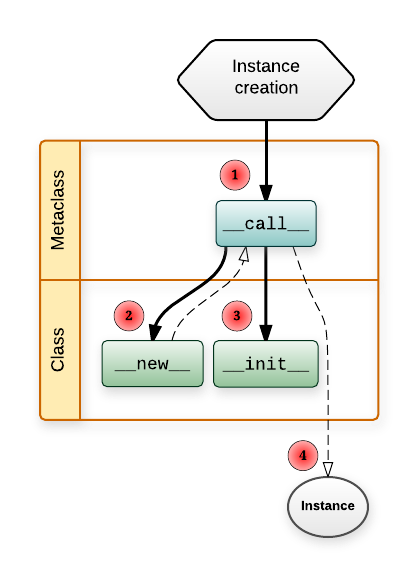
\includegraphics[width=0.7\onepicwidth]{figure/var/instance-creation}
        \caption{The diagram of how instances are constructed.\footnote{
                 \href{https://blog.ionelmc.ro/2015/02/09/understanding-python-metaclasses/}{Understanding Python metaclasses}}}
    \end{figure}
\end{frame}

\begin{frame}[fragile]
    \begin{tcblisting}{title=code snippe of tf 2.0 Variable}
            class VariableMetaclass(type):
              def _variable_v1_call(cls, **kwargs):
                pass

              def _variable_v2_call(cls, **kwargs):
                pass

              def __call__(cls, *args, **kwargs):
                if cls is VariableV1:
                  return cls._variable_v1_call(*args, **kwargs)
                elif cls is Variable:
                  return cls._variable_v2_call(*args, **kwargs)
                else:
                  return super(VariableMetaclass, cls).__call__(*args, **kwargs)

            @tf_export("Variable", v1=[])
            class Variable(six.with_metaclass(VariableMetaclass,
                                              checkpointable.CheckpointableBase)):
              def __init__(self, **kwargs):
                raise NotImplementedError
    \end{tcblisting}
    {\tiny \tt
    source: tensorflow/python/ops/variables.py \\[-2ex]
    commit: 4a5693e732b80a593bca7bf94ddd5df9e5d78cc0}
\end{frame}

% -*- coding: utf-8 -*-

\subsection{tf.print}
\begin{frame}{主要变动}
    similar to the standard python print API.\footnote{\href{https://github.com/tensorflow/community/pull/14}{RFC: New tf.print}}


    \begin{itemize}
        \item tf.Print $\to$ tf.print, tf.strings.format
            \begin{itemize}
                \item For python 2: \lstinline{from __future__ import print_function}
            \end{itemize}
        \item identity op $\to$ control dependencies
        \item controllable logging levels
            \begin{itemize}
                \item stdout/sterr,与notebook不兼容
                \item device: cpu:0 by default?
            \end{itemize}
        \item supports for nested data structures
    \end{itemize}
\end{frame}

\begin{frame}[fragile]
\begin{lstlisting}[language=Python,style=myScalastyle, caption=eager mode]
tf.enable_eager_execution()
tensor = tf.range(10)
tf.print(tensor, output_stream=sys.stderr)
# (This prints "[0 1 2 ... 7 8 9]" to sys.stderr)
\end{lstlisting}

\begin{lstlisting}[language=Python,style=myScalastyle, caption=graph mode]
with sess.as_default():
  tensor = tf.range(10)
  print_op = tf.print(tensor, output_stream=sys.stdout)
  # For tf 1.0: return an identity op:
  # doubled_tensor = print_op * 2
  # For tf 2.0:
  with tf.control_dependencies([print_op]):
    doubled_tensor = tensor * 2
  sess.run(doubled_tensor)
  # (This prints "[0 1 2 ... 7 8 9]" to sys.stdout)
\end{lstlisting}
\end{frame}

% -*- coding: utf-8 -*-

\subsection{RNN}

\begin{frame}{Unify RNN interface}
    Unify the final API that is similar to existing Keras API, and port functionalities from TF RNN to Keras.\footnote{\href{https://github.com/tensorflow/community/pull/15/}{RFC: Unify RNN interface}}

    \begin{itemize}
        \item gate order: IFCO vs ICFO
        \item tf.contrib.rnn: 只迁移少部份RNN Cell
        \item NVidia CuDNN
    \end{itemize}

\end{frame}

% -*- coding: utf-8 -*-

\subsection{namespaces}

\begin{frame}{namespaces}
    structure namespaces in a clear way for easier discoverability and usability.\footnote{\href{https://github.com/tensorflow/community/pull/16}{RFC: TensorFlow API symbols and namespaces}}

    \begin{itemize}
        \item \lstinline{tf_export} decorator
        \item additional namespaces
            \begin{itemize}
                \item tf.losses $\to$ tf.keras.losses
                \item tf.metrics $\to$ tf.keras.metrics
                \item tf.layers $\to$ tf.keras.layers
            \end{itemize}
        \item deprecated namespaces
            \begin{itemize}
                \item tf.logging $\to$ Python logging module
                \item tf.manip: keep them in root instead.
            \end{itemize}
    \end{itemize}
\end{frame}

% -*- coding: utf-8 -*-

\subsection{collections}

\begin{frame}
    主要用法:
    \begin{description}
        \item[搜索汇总]  用户自行收集和追踪
            \begin{itemize}
                \item queue runner $\to$ tf.data
                \item variable $\to$ 利用variable creator在创建时追踪
                \item update op $\to$ 在model\_fn里更新,或者用keras的model.updates
            \end{itemize}
        \item[序列化]    SaveModel,后续会有专门API支持
        \item[维持状态]  SharedEmbeddingColumns,使用全局变量替代
    \end{description}
\end{frame}

\begin{frame}[fragile]
    \begin{tcblisting}{title=VariableTracker example}
            class VariableTracker(object):
              def __init__(self):
                self.variables = []

              def variable_tracker(self, next_creator, **kwargs):
                v = next_creator(**kwargs)
                self.variables.append(v)
                return v

            with tf.variable_creator_scope(tracker.variable_tracker):
              # ...
              a = tf.Variable(0)
              # ...
            assert tracker.variables == [a]
    \end{tcblisting}
\end{frame}

% -*- coding: utf-8 -*-

\section{tf.contrib}

\begin{frame}{tf.contrib}
    sunset the present tf.contrib, and replace its important functions with more maintainable alternatives.\footnote{\href{https://github.com/tensorflow/community/pull/18}{RFC: Sunset tf.contrib}}

    \begin{itemize}
        \item moving to core: symbols should be prefixed with experimental.
        \item moving to a seperate repository
            \begin{itemize}
                \item tensorflow/addons: layer, metric, loss, optimizer, op or kernel
                \item tensorflow/network (IO?)
                \item tensorflow/scientific
            \end{itemize}
        \item deleting
    \end{itemize}
\end{frame}

%% -*- coding: utf-8 -*-

\section{functions}

\begin{frame}
\end{frame}

%% -*- coding: utf-8 -*-

\section{总结}
\begin{frame}{总结}
% 发展史
%% PPT, a little history
%% http://blog.flynn.wang/sharing/an_introduction_to_GBDT_and_XGBoost.pdf
\end{frame}


% 添加你的其他文件


% 封底
\createlastpage

\end{document}
% 文末
